\chapter{Problem}\label{chap:problem}
\acrfull{IoT} devices get rapidly more and more integrated in our daily life \cite{Yu2017}. In fact, the number of IoT devices are expected to almost triple until 2030 accordingly to a statistic from Statista in cooperation with Transform Insights  \cite{StatisticTransformaInsights} \cite{StatisticTransformaInsightsByUseCase}. Figure \ref{fig:mumber_of_iot_devices} shows this statistic, which indicates the rapid increase in connected IoT devices around the world. In 2020 60\% of all IoT devices belong to the consumer segment \cite{StatisticTransformaInsightsByUseCase}.

\begin{figure}[H]
    \centering
    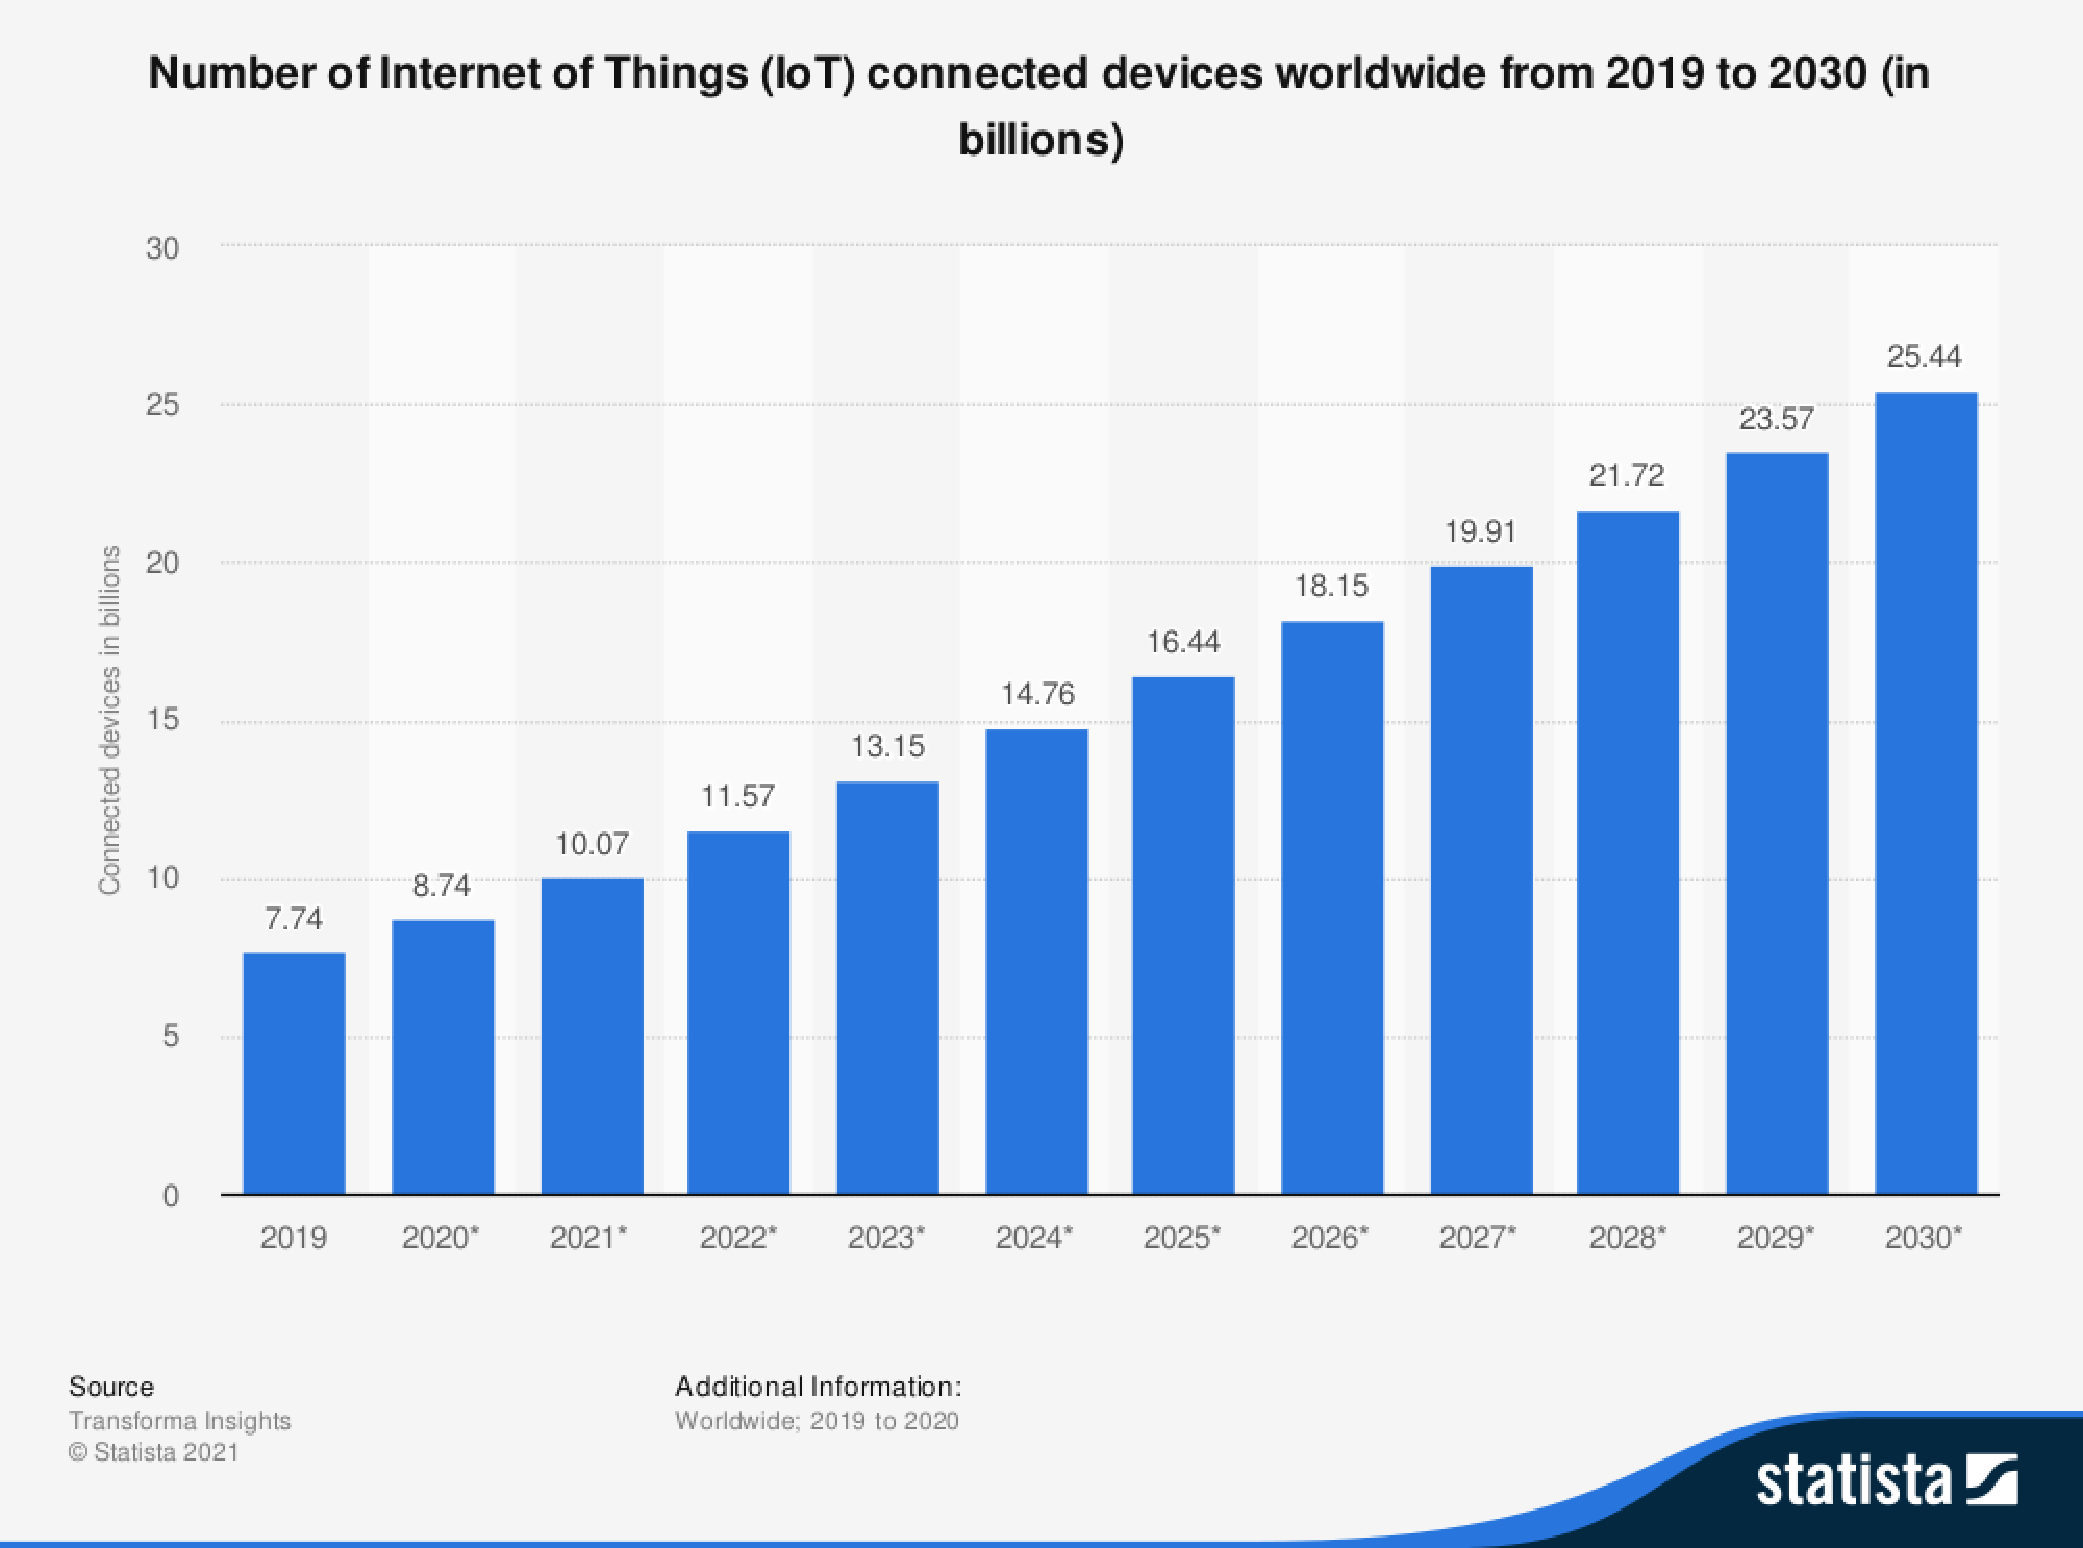
\includegraphics[width=0.8\textwidth]{assets/problem/statistic_id1183457_number-of-iot-connected-devices-worldwide-2019-2030.pdf}
    \caption{Number of IoT devices \cite{StatisticTransformaInsights}.}\label{fig:mumber_of_iot_devices}
\end{figure}

With the increasing amount of connected IoT devices, the data production increases too. Increase in data production also increases the demand to process the generated datasets. One conventional way  is the processing through cloud computing services. But this process generates significantly more pressure on the overall network and its bandwidth with increasing number of devices \cite{Yu2017}. For example, transmitting 1080p Video streams, in real time, from around 12,000 different devices requires a cloud ingress bandwidth of 100 gigabits per second. One million of these devices require 8.5 terabits per second. Sending the video streams to nearby processing platforms like edge computing platforms will reduce the overall bandwidth congestion \cite{Shi2016a}. 

\bigskip
Advantages like almost infinite computing power, unlimited storage capacity, dynamically scale your services or the fact of only paying what you use, the so-called pay-as-you-go model, has driven many businesses to migrate to centralized cloud approaches \cite{APOSTU2013}. Edge Computing on the other hand is a decentralized computing infrastructure. Disadvantages from cloud computing like privacy, security or compliance come out as a benefit on edge computing \cite{IndustrialInternetConsortium2018}. For example, edge computing infrastructures can enforce privacy policies of its owner by keeping the data inside the users trust domain\cite{Shi2016a}. Other advantages like masking cloud outages \cite{Shi2016a} can be also a benefit of moving to the edge. For example the recent incident at OVH Cloud in France destroyed an entire data center due to a fire, which resulted in an irreversible data loss for many businesses at once \cite{Holland2021}. Outages like the fire or other outages like network failures, denial-of-service attacks (DDoS) and more do not affect local edge computing infrastructures \cite{Shi2016a}. But more about the advantages of edge computing in the chapter \ref{chap:edge-computing}. 

\bigskip
Also, round trip times (RTT) to remote data centers are increased compared to local computation units. The most obvious about increased RTT is the physical distance. There is no way to get around the speed of light limitation. Another limiting factor is the node count and the congestion on each of the nodes the connection takes on its way \cite{Cloudflarea}. An example where high latency can be a problem are offshore oil rigs. Connecting oil rigs to the internet with under sea cables won’t be a financially viable option for the operators. Satellite connectivity is used to transfer data from oil rigs to the mainland \cite{HaglandHansen}. The RTT over satellite was measured to be around 880ms to 1243ms \cite{Bisu2018}. This high latency may be improved in the future by newer satellite installations like SpaceX’s Starlink constellation which aims to be as low as 20-40ms RTT. Starlink constellation is currently in a public beta testing phase \cite{Grush2020}. Latency is also affected by the bandwidth of each line between the nodes taken by the connection. The line with the smallest bandwidth is referred to as the bottleneck bandwidth. The rate of sending at the bottleneck affects the overall latency. The bottleneck bandwidth also indicates the maximum possible throughput \cite{Gettys2011}. The latency and bandwidth limits can be partially masked with sufficient effort and resource investment, like setting up a direct fiber cable connection to the nearest data center \cite{Shi2016a}.

\bigskip
One potential new requirement for some IoT devices is the near real-time capability, which is only possible due to the decrease in response time by a shorter traveling distance inside the system environment. A real life example of a big amount of data which needs to be processed near real time is the rise of the autonomous vehicle. Each of these autonomous vehicles has a lot of sensors and cameras on board whose data must be processed near real time to perform an appropriate response to the surrounding environment. Sending this data into the cloud as an unbound latency, hence we can not implement near real time application with a cloud component. Edge computing targets this need of processing data locally. No wonder that a number of commercial and open source edge platforms are out there to be chosen. 

\bigskip
To Sum it up so-called edge platforms can be used to simplify the distribution of workloads on the edge to meet the given requirements which the cloud and remote data centers can’t meet. 
